\documentclass{article}

% set font encoding for PDFLaTeX or XeLaTeX
\usepackage{ifxetex}
\ifxetex
  \usepackage{fontspec}
\else
  \usepackage[T1]{fontenc}
  \usepackage[utf8]{inputenc}
  \usepackage{lmodern}
   \usepackage{graphicx}
  \usepackage{float}
\fi

% used in maketitle
\title{Reporte Actividad 2}
\author{Eduardo Hndz}

% Enable SageTeX to run SageMath code right inside this LaTeX file.
% documentation: http://mirrors.ctan.org/macros/latex/contrib/sagetex/sagetexpackage.pdf
% \usepackage{sagetex}

\begin{document}
\maketitle
\section{Introducción}
En esta sección aprendimos a usar la plataforma web \textbf{Jupyter Notebook} la cual es un entorno de programación en el cual podemos interactuar con lenguajes de programación como \textbf{Python} y \textbf{R}.


\section{Jupyter Notebook}
La plataforma en linea Jupyter es un sitio donde puede trabajar con Python y R. \\
Hasta ahora nosotros aprendimos a utilizar Python, en el cual necesitamos de tres librerías principales, las cuales son las siguientes  $:$
\begin{itemize}
\item \textbf{Pandas:} Pandas es un paquete de Python que proporciona estructuras de datos rápidas, flexibles y expresivas  diseñadas para que el trabajo con  datos \textbf{relacionales} o \textbf{etiquetados} sea fácil o intuitivo.
\item \textbf{NumPy:} NumPy es el paquete fundamental para la programación con Python.
Su uso principal es el de un almacenamiento multidimensional eficiente de datos genéricos.
\item \textbf{Matplotlib.Pyplot:} Matplotlib es una biblioteca de bosquejo en Python que produce figuras en una variedad de formatos impresos y entornos interactivos en todas la plataformas.\\
Matplotlib intenta hacer las cosas fáciles.\\
se pueden generar gráficos, histogramas, espectros de potencia,gráficos de barras,diagramas de caja, diagramas de dispersión, etc.
\end{itemize}
\section{Limitaciones}
A opinión propia las limitaciones que encontré fue la necesidad de resetear el kernel, al parecer, después de relizar intentos con comandos distintos el sitio web se crashea, provocando la necesidad de reiniciar el kernel.
\section{Actividad}
El profesor nos otorgó un código de python el cual fuimos copiando renglón por renglón\\
El primer comando nos sirvió para agregar  la librería de pandas,numpy y matplot
posteriormente tuvimos que ingresar a la página del servicio meterológico nacional , elegimos una estación de nuestra preferencia y procedimos a descargar los datos de un día.\\
una vez descargados los datos usamos el comando \textit{$pd.read_csv$} para leer el archivo con los datos descargados.\\
Después realizamos un análisis de datos con el comando \textit{head()} el cual nos muestra los primeros 5 datos del archivo, dimos estructura con \textit{$pd.DataFrame()$}
e identificamos el tipo de datos que teníamos con \textit{dtype}\\
una vez realizado eso, el profesor nos explicó que debíamos mover la columna de fecha al final y además agregarle la hora a éste.
%aquí va la imagen del renglon
\begin{figure}[h!]
\centering
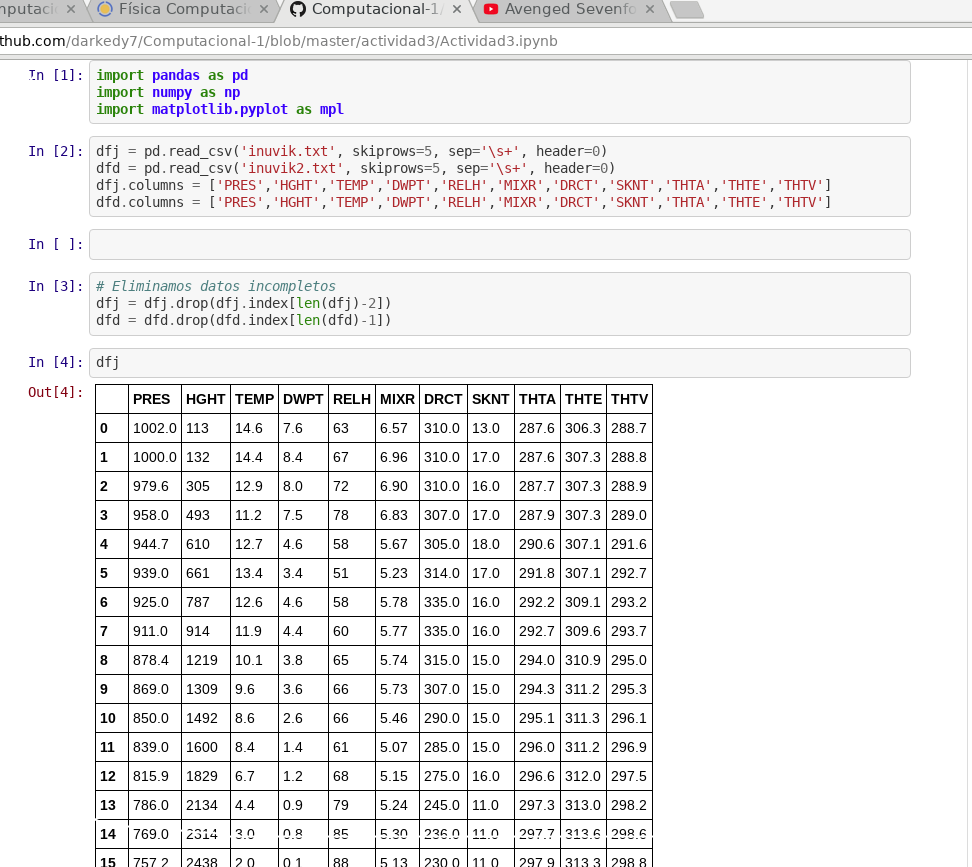
\includegraphics[width=10.0cm,height=10.0cm]{1.png}
\end{figure}
\\aprendimos a seleccionar datos que necesitáramos (datos con características específicas) y a calcular el promedio con \textit{mean}, el cual obtenía el promedio de todos los datos de tipo numérico.\\

Posteriormente realizamos gráficas :
\begin{itemize}
\item \textbf{De un solo dato:}
\begin{figure}[h!]
\centering
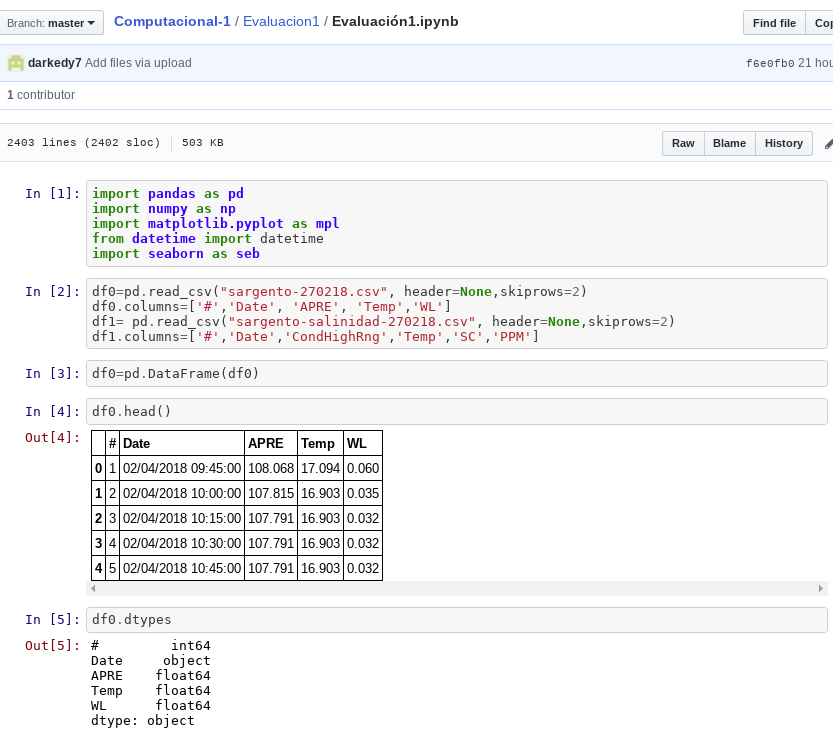
\includegraphics[width=15.0cm,height=10.0cm]{2.png}
\end{figure}
\newpage
\item \textbf{De dos datos Vs tiempo}
\begin{figure}[h!]
\centering
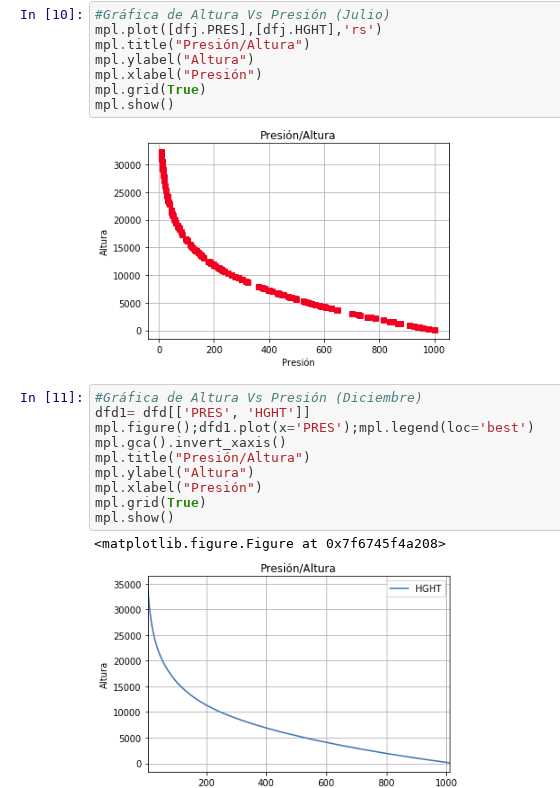
\includegraphics[width=15.0cm,height=10.0cm]{3.png}
\end{figure}
\newpage
\item \textbf{Agregando Límetes}
\begin{figure}[h!]
\centering
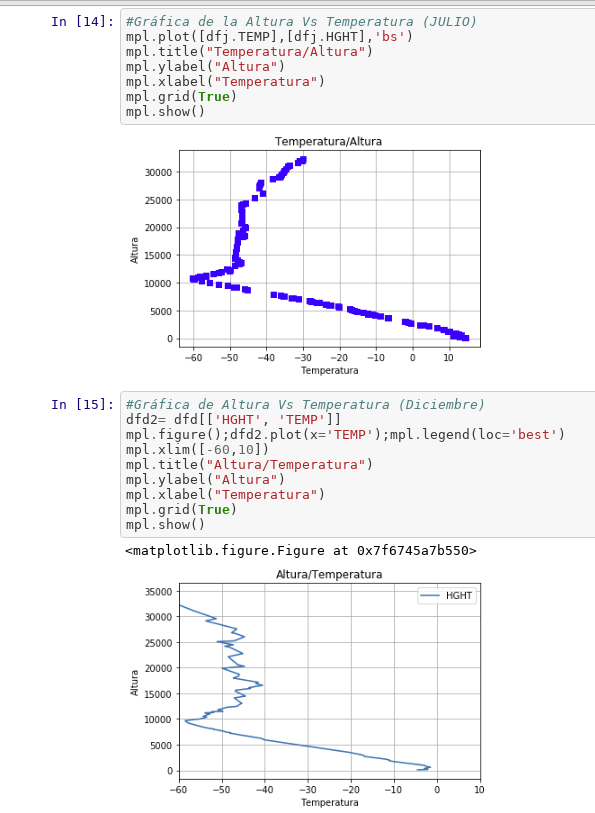
\includegraphics[width=15.0cm,height=8.0cm]{4.png}
\end{figure}
\end{itemize}

\section{Apéndice}
\begin{enumerate}

\item {¿Cuál es tu primera impresión de Jupyter Notebook?}\\
Jupyter es un poco difícil de utilizar al inicio, pero al aprender el significado de cada comando comienza a facilitar su uso.

\item {¿Se te dificultó leer código en Python?}\\
Un poco la verdad, creí sería un poco más fácil, tengo problemas en lo que es la graficación.
\item{¿En base a tu experiencia de programación en Fortran, que te parece el entorno de trabajar en Python?}\\
Interesante, es muy distinto a fortran a lo que he visto ahora. la facilidad es que puedes agregar bibliotecas para realizar actividades extras en el mismo lugar.

\item{A diferencia de Fortran, ahora se producen las gráficas utilizando la biblioteca Matplotlib. ¿Cómo fue tu experiencia?}\\
Entretenida y eficaz, siento que es más fácil graficar en python.

\item {En general, ¿qué te pereció el entorno de trabajo en Python?}\\
Es interesante, un entorno muy completo pero a su vez complejo.

\item {¿Qué opinas de la actividad?}\\
Fue entretenida  necesaria
\item{¿Estuvo compleja?}\\
Sí.
\item{¿Mucho material nuevo?}\\
Hasta ahora creo que fue el necesario.
\item{¿Que le faltó o que le sobró?}\\
Tiempo.
\item{¿Qué modificarías para mejorar?}\\
En la actividad nada, solo ser más autodidacta
\end{enumerate}

\end{document}
